\section{Aufbau}\label{sec:aufbau}

\subsection{Klassenstruktur}\label{subsec:klassenstruktur}
\begin{center}
    \makebox[\textwidth][c]{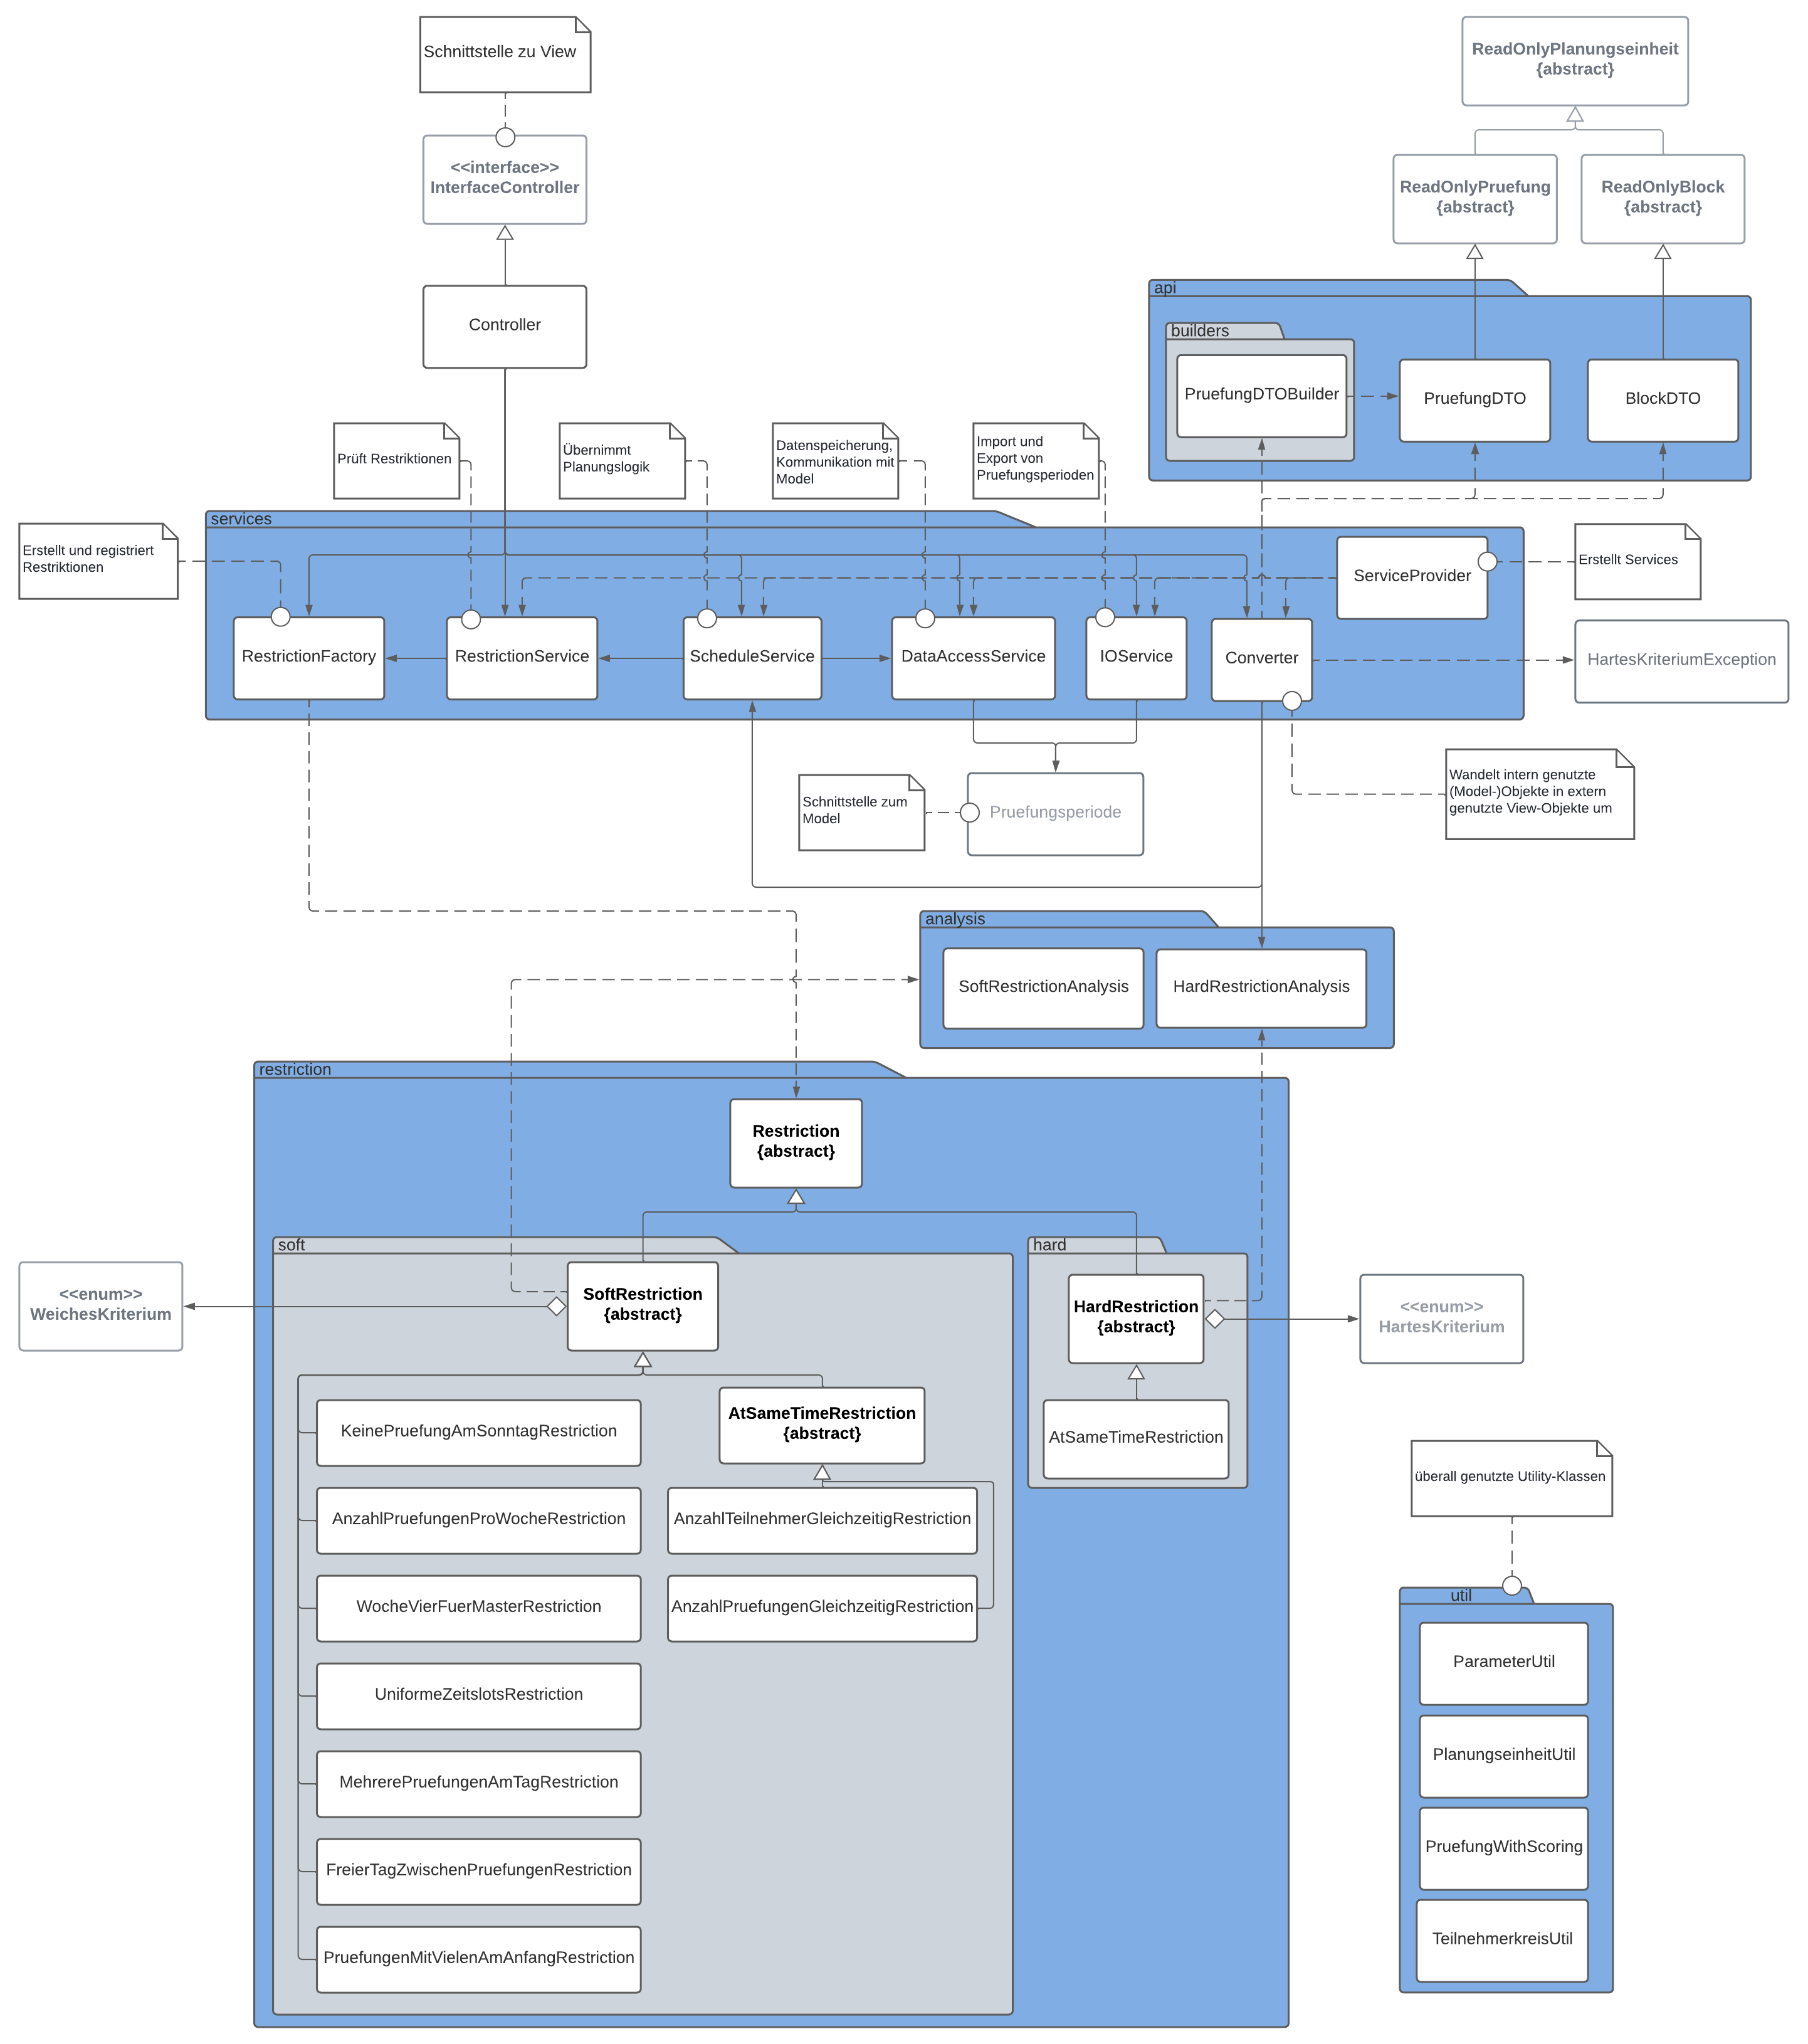
\includegraphics[width=1.25\textwidth]{extra/controller_2_uml}}%
\end{center}

\clearpage
Den Einstieg des Projekts von View-Seite bildet die Klasse \enquote{Controller}.
Das Projekt selbst gliedert sich in fünf Haupt-Pakete, wobei sich die Hauptfunktionalität
auf die Pakete \enquote{services} und \enquote{restriction} beschränkt.

Die einzelnen Services dienen der logischen Trennung der im Controller angebotenen Funktionalität.
Während der~\nameref{subsec:dataaccessservice} sich beispielsweise auf die Kommunikation mit dem Model fokussiert,
werden im~\nameref{subsec:ScheduleService} alle Planungen vorgenommen.
Genauere Beschreibungen zu den Services finden sich im Abschnitt\nameref{sec:Services}.
Das Package \enquote{restriction} beinhalten alle Restriktionen, die für das Planen von Prüfungen
und Blöcken ausgewertet werden (siehe~\nameref{sec:restrictions}).

Neben dem Paket~\enquote{util}, welches Hilfsklassen beinhaltet, gibt es außerdem das Package \enquote{api}
in dem sich Implementierungen der ReadOnly-Klassen finden, die für die Kommunikation mit View dienen
und das Package~\enquote{analysis}, das Klassen zur internen Kommunikation von Restriktions-Auswertungen enthält.
\pagebreak
\subsection{Aufbau der Scoring-Berechnung}\label{subsec:aufbau-der-scoring-berechnung}
\begin{figure}[!h]
    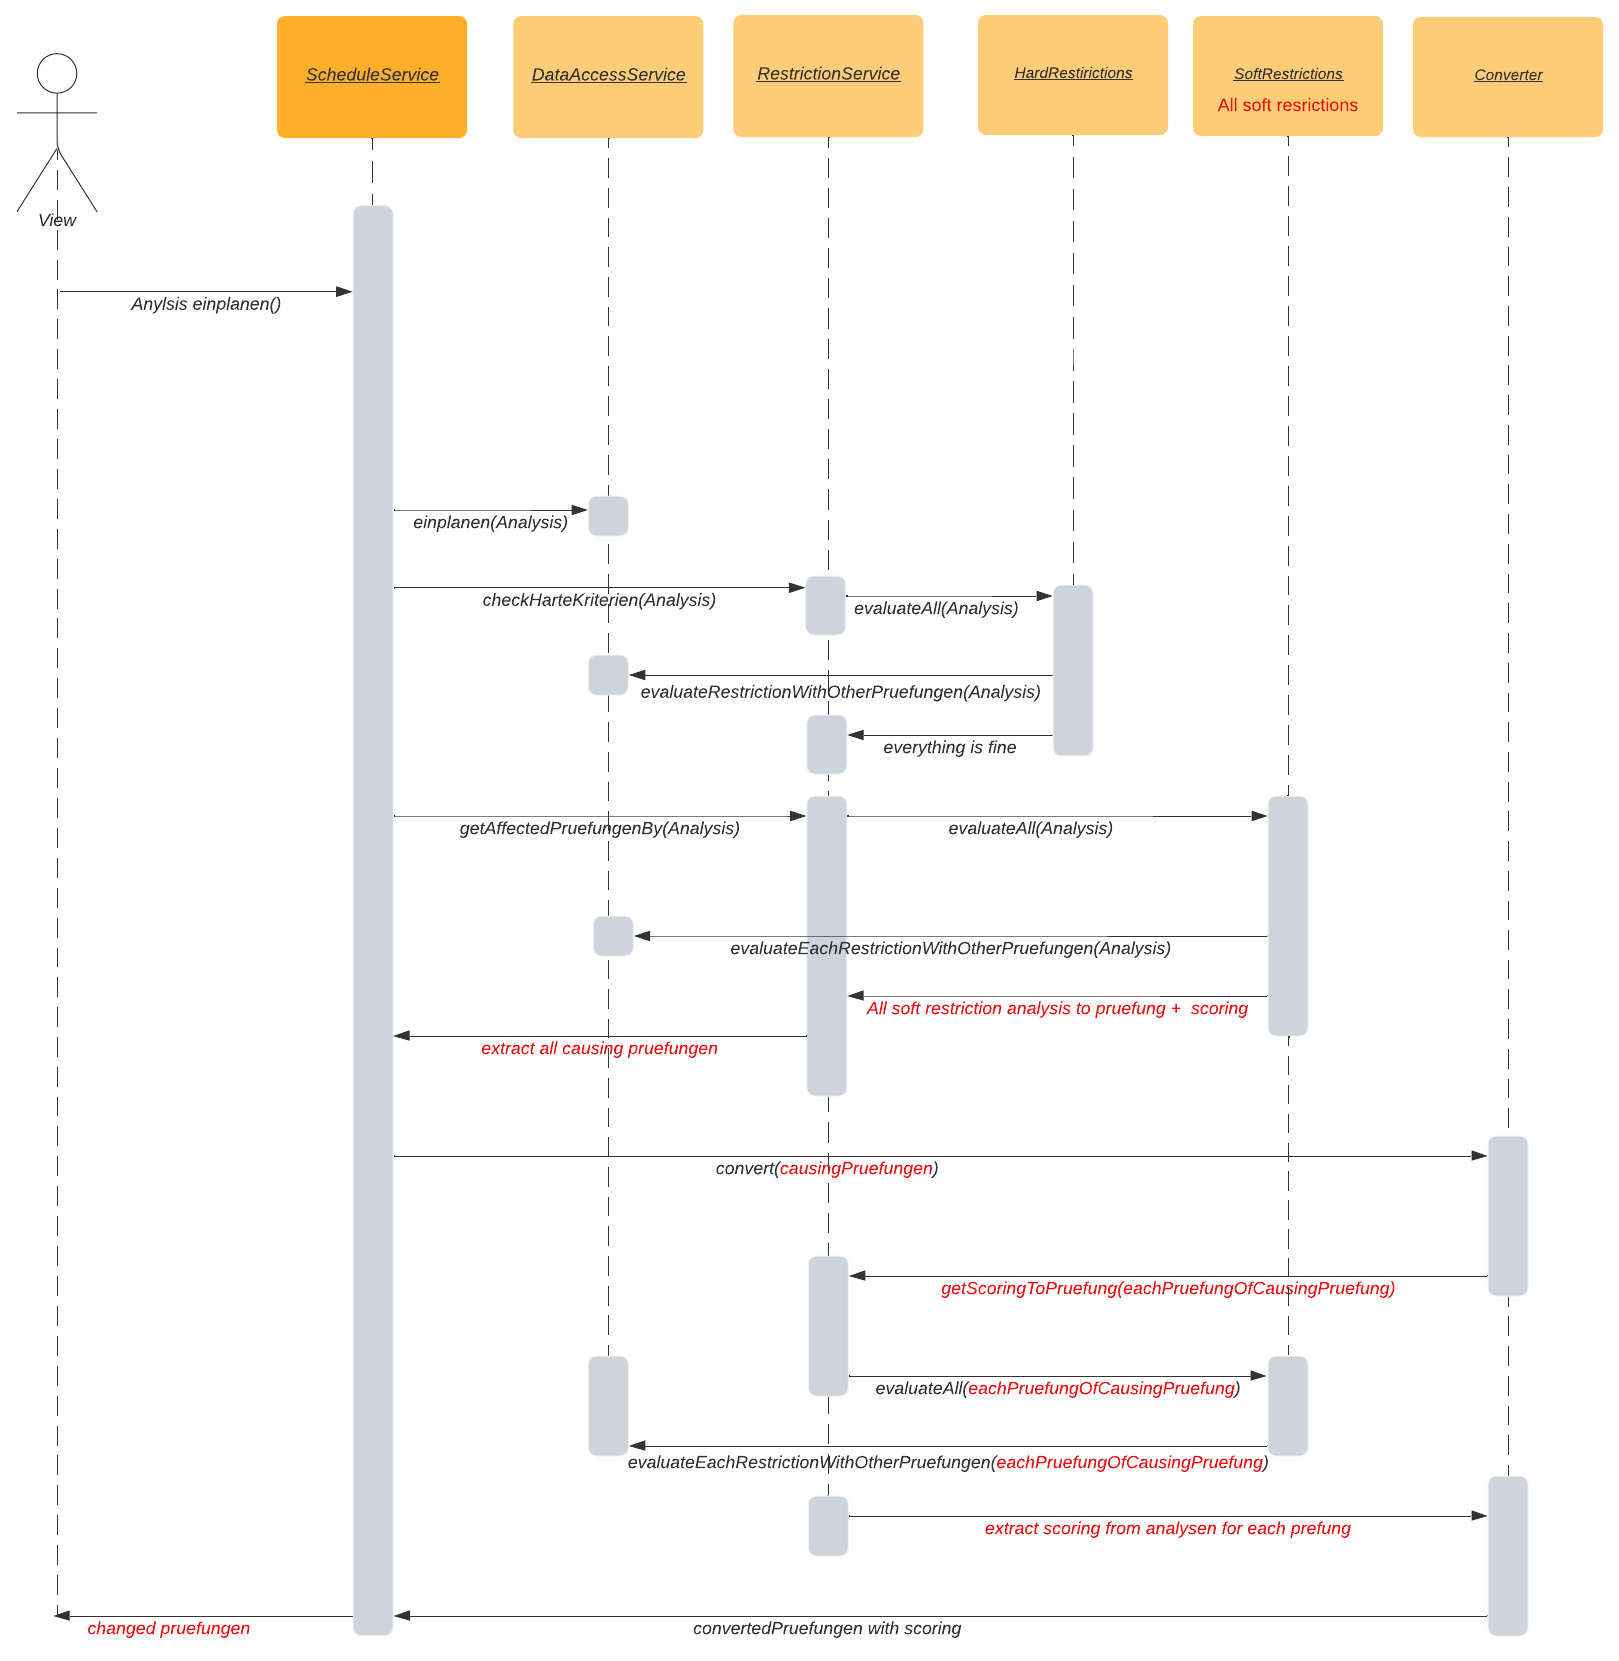
\includegraphics[width=0.9\textwidth]{extra/Sequence_diagram}\label{fig:figure}
\end{figure}

Im Sequenzdiagramm wird ein beispielhaftes Einplanen der Prüfung Analysis dargestellt.
Das Scoring zu einer Prüfung wird dadurch berechnet, dass jede weiche Restriktion ausgewertet und in
einer Analyse für weiche Kriterien zusammengefasst wird.
Jede Restriktion evaluiert dabei unterschiedlich, da für manche Kriterien z.B.\ das Vorhandensein weiterer
Pruefungen oder die Anzahl von betroffenen Teilnehmern in das Analyseergebnis eingehen.
Dabei können auch bereits geplante Prüfungen zur Evaluierung herangezogen werden.
Die Analyse eines Kriteriums bezieht sich jeweils auf genau eine Pruefung.
Die Summe der Teilscorings aus den Analysen ergibt das Gesamtscoring einer Pruefung.
